\documentclass[tikz, margin=2mm]{standalone}

\begin{document}
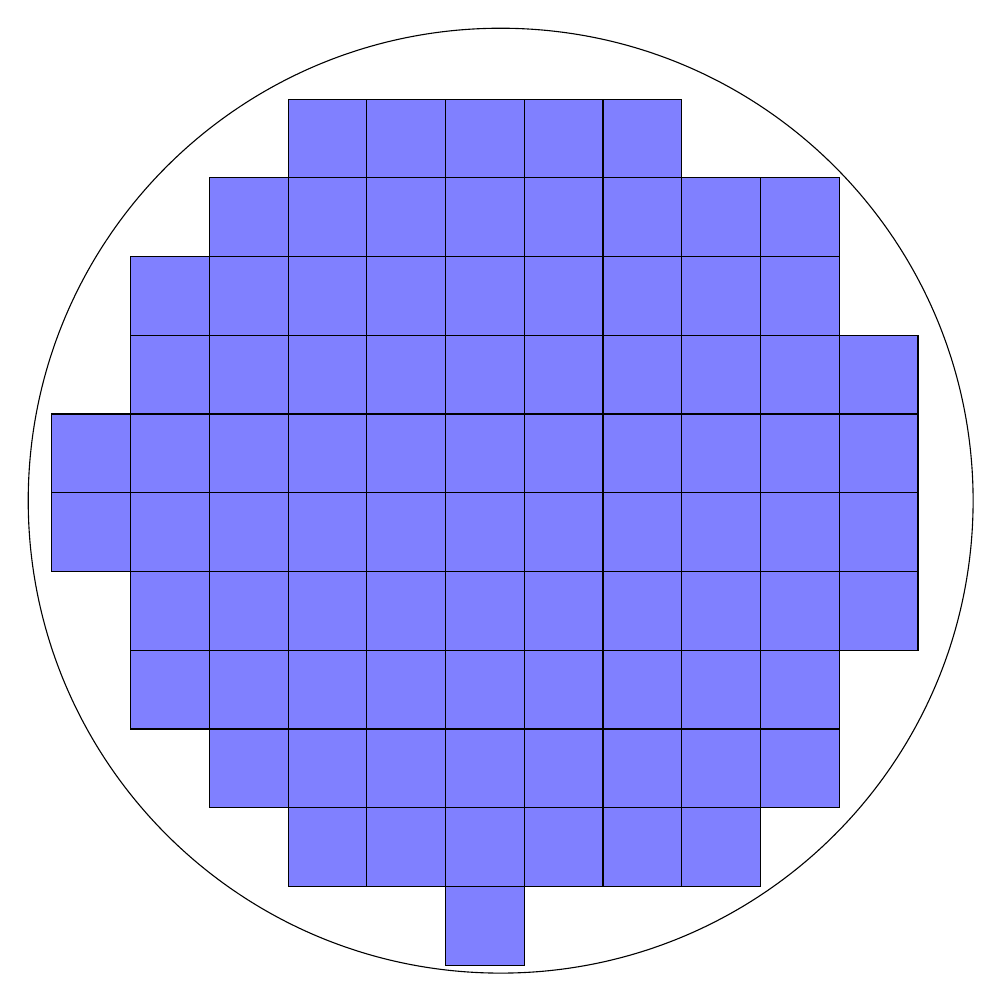
\begin{tikzpicture}
    \def\radius{6}
    \def\squaresXshift{.3}
    \def\squaresYshift{.1}
    \foreach \x [evaluate=\x as \xp using {\x+\squaresXshift}] in {-\radius,...,\radius} {
        \foreach \y [evaluate=\y as \yp using {\y+\squaresYshift}] in {-\radius,...,\radius} {
            \pgfmathparse{
                (\xp+1)^2 + (\yp+1)^2 <= \radius^2 &&
                (\xp+1)^2 + (\yp)^2   <= \radius^2 &&
                (\xp)^2   + (\yp+1)^2 <= \radius^2 &&
                (\xp)^2   + (\yp)^2   <= \radius^2
            } %Condition of squares to stay inside the circle. 
            %This circle is translated to make it work.
            \ifnum\pgfmathresult=1
                \filldraw[fill=blue!50] (\xp,\yp) rectangle ++(1,1); %Colouring the squares
            \fi
        }
    }
    \draw (0,0) circle [radius=\radius]; %Circle
\end{tikzpicture}
\end{document}